
\documentclass[a4paper]{article}
\usepackage[pdftex]{graphicx}
\usepackage[utf8]{inputenc}
\usepackage{enumerate}
\usepackage{siunitx}
\sisetup{locale=DE} 
\usepackage{icomma}
\usepackage{amssymb}
\usepackage{tikz}
\usepackage{href-ul}
\hypersetup{
	colorlinks=true,
	linkcolor=blue,
	urlcolor=blue}
\usepackage{geometry}
\geometry{a4paper, top=15mm, left=15mm, right=15mm, bottom=15mm,
	headsep=10mm, footskip=12mm}

\begin{document}
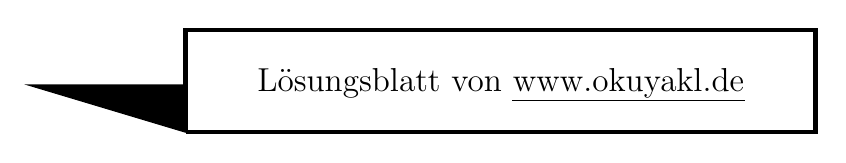
\begin{tikzpicture}(10,3)
	\draw[ultra thick](2,0) --(10,0) -- (10,1.3) --(2,1.3) -- (2,0);
	\draw[fill=black](2,0)-- (0,.6) -- (2,.6) -- (2,0);
	\node at (6,.6) {\large Lösungsblatt von \href{https://www.okuyakl.de}{www.okuyakl.de}};
\end{tikzpicture}
\vspace{0.5 cm}


\noindent{\bf Aufgabe 1. a)}\\
Es sind dies Leiterkennlinien

\begin{itemize}
\item 1: Bleistiftmine. Bei steigendem Stromfluss nimmt die Temperatur zu, die Leitfähigkeit nimmt dabei zu, die Kurve steigt an.
\item 2: Eisendraht. Bei steigendem Stromfluss nimmt die Temperatur zu, die Leitfähigkeit nimmt dabei ab, die Kurve flacht ab.
\item 3: Konstantandraht. Die Leitfähigkeit ist unabhängig von der Temperatur. Steigung bleibt konstant.
\end{itemize}
\vspace{0.5 cm}

\noindent{\bf Aufgabe 1. b)}\\
Bei $\SI{4}{\volt}$ zeigt der Leiter aus Eisen den höchsten Stromfluss. Wir lesen ab: $I =\SI{1,2}{\ampere}$
Damit ist der elektrische Widerstand dieses Leiterstücks:
$$R={U \over I} = {\SI{4,0}{\volt} \over \SI{1,2}{\ampere}}\approx \SI{3,3}{\ohm}$$ 
\vspace{0.5 cm}

\noindent{\bf Aufgabe 1. c)}\\
Bei steigender Spannung erwärmt sich der Eisendraht. Im Atomgitter des Eisens schwingen die Atomrümpfe nun stärker und stellen sich den fließenden Elektronen vermehrt in den Weg. Der Widerstand steigt.
\vspace{0.5 cm}

\noindent{\bf Aufgabe 1. d)}\\
\begin{itemize}
	\item Ein Kaltleiter ist ein PTC, das heißt positive temperature coefficient. Dieser leitet bei tiefen Temperaturen besser. 
	\item Ein Heißleiter ist ein NTC, das heißt negative temperature coefficient.
	Dieser leitet bei hohen Temperaturen besser.
\end{itemize}
\vspace{0.5 cm}

\noindent{\bf Aufgabe 2. a)}\\
\renewcommand{\arraystretch}{1.5}
\begin{tabular}{cccccccc}
$U$ in V & 0 & 1,8 & 3,6 & 5,4 & 7,2 & 9,0 & 10,8 \\
\hline
$I$ in A & 0 & 0,31 & 0,55 & 0,74 & 0,84 & 0,93 & 0,96 \\
$R$ in $\SI{}{\ohm}$ & - & 5,8 & 6,5 & 7,3 & 8,6 & 9,7 & 11  
\end{tabular}

\noindent
Bei Leiter 1 ist deutlich die Zunahme des Widerstands bei steigendem Stromfluss zu erkennen.
\vspace{0.5 cm}

\noindent
\begin{minipage}{0.5\textwidth}
	\noindent{\bf Aufgabe 2. b)}\\
	Die Steigung des Graphen ist überall gleich. Das bedeutet, dass das Verhältnis von Spannung zu Strom, der Widerstand $R$ immer gleich bleibt. 
	\vspace{0.5 cm}
	
	\noindent{\bf Aufgabe 2. c)}\\
	Leiter 1 leitet bei Kälte besser, bei Leiter 2 spielt die Temperatur für den Widerstand keine Rolle. Der Widerstand von Leiter 2 ist konstant $\SI{10}{\ohm}$. 
	\vspace{0.5 cm}
	
	\noindent{\bf Aufgabe 3. a)}\\
	Der Widerstand errechnet sich mit:
	$$R={U\over I} = {\SI{6,0}{\volt} \over \SI{5,0}{\ampere}}=\SI{1,2}{\ohm}$$
\end{minipage}
\hspace{1 cm}
\begin{minipage}{0.5\textwidth}
	\includegraphics[width=7 cm]{beleik185}
\end{minipage}
\vspace{0.5 cm}

\noindent{\bf Aufgabe 3. b)}\\
Wir wenden wieder das Ohm'sche Gesetz an und erhalten:
$$U = R \cdot I = \SI{50}{\ohm} \cdot \SI{0,38}{\ampere} = \SI{19}{\volt}$$
\vspace{0.5 cm}

\noindent

	\noindent{\bf Aufgabe 3. c)}\\
	Die Elektrische Leistung ist:
	$$P = U \cdot I \quad \Rightarrow \quad I = {P \over U} = {\SI{40}{\watt} \over \SI{230}{\volt}}=\SI{0,17}{\ampere}$$
	Der Widerstand ist somit:
	$$R = {U \over I} = {U^2 \over P} = {(\SI{230}{\volt})^2\over \SI{40}{\watt}}=\SI{1,3}{\kilo\ohm}$$
	
	\vspace{0.5 cm}
	
	\noindent{\bf Aufgabe 3. d)}\\
	Wieder ist:
	$$U = R \cdot I = \SI{1000}{\ohm} \cdot \SI{0,015}{\ampere} = \SI{15}{\volt}$$
\begin{center}
	\includegraphics[width=7 cm]{../../viecher/endcomic.pdf}
	
	Hier geht es zurück zum \href{https://www.okuyakl.de/phys/p8widL185/aa185.pdf}{Aufgabenblatt}
\end{center}

\end{document}